\documentclass[a4paper,12pt]{article}   % papír A4, písmo 12 bodu
\usepackage[czech]{babel}               %podpora cestiny
\usepackage[T1]{fontenc}                %pouzij variantu pisma T1 (hacky, carky)

\usepackage[utf8x]{inputenc}            %kodovaní UTF-8
\usepackage{ucs}                        %kodovani unicode

\usepackage[left=2.5cm,right=2.5cm,top=2.5cm,bottom=2.5cm]{geometry} %okraje stranky
\usepackage{amsmath,amsfonts,amssymb}   %podpora matematiky
\usepackage{gensymb,marvosym}           %symboly celsius (\celsius) apod.
\usepackage{times}                      %font Times New Roman (matematika pismem Computer Modern) 
\usepackage{parskip}                    %mezera mezi odstavci
\usepackage[none]{hyphenat} \sloppy     %slova nedelit a~nepretekat
\usepackage{titlesec}                   %hlubsi nastaveni nadpisů
\setcounter{secnumdepth}{4}
\clubpenalty 10000                      %kontrolovat sirotky
\widowpenalty 10000                     %kontrolovat vdovy
\usepackage{array}
\usepackage{setspace} \onehalfspacing   %podpora pro zmenu radkovani + radkovani 1,5
\usepackage{enumerate}                  %podpora pro zmenu cislovani
\usepackage{fancyhdr}                   %vlastni zahlavi a~zapati
\usepackage{graphicx}                   %podpora grafiky
\graphicspath{{figures/}}               %vychozi adresar s~obrazky
\usepackage{caption}                    %popisky
\usepackage{subcaption}                 %podpopisky
\usepackage{siunitx}
\usepackage[shortlabels]{enumitem}
\usepackage{lastpage}                   %zjištění poslední stránky \pageref{LastPage}
\usepackage{float}                      
\usepackage{url}
\usepackage[unicode]{hyperref}          %klikaci odkazy v textu
\usepackage{multirow}
\usepackage[percent]{overpic}
\usepackage{lipsum}


\usepackage{halloweenmath}


\titleclass{\subsubsubsection}{straight}[\subsection]
\newcounter{subsubsubsection}[subsubsection]
\renewcommand\thesubsubsubsection{\thesubsubsection.\arabic{subsubsubsection}}
\renewcommand\theparagraph{\thesubsubsubsection.\arabic{paragraph}} % optional, useful if paragraphs are to be numbered


%------------------------ čtvrtá a~pátá úroveň nadpisu ---------------------------

\titleformat{\subsubsubsection}
  {\normalfont\normalsize\bfseries}{\thesubsubsubsection}{1em}{}
\titlespacing*{\subsubsubsection}
{0pt}{3.25ex plus 1ex minus .2ex}{1.5ex plus .2ex}

\makeatletter

\renewcommand\paragraph{\@startsection{paragraph}{5}{\z@}%
  {3.25ex \@plus1ex \@minus.2ex}%
  {-1em}%
  {\normalfont\normalsize\bfseries}}
\renewcommand\subparagraph{\@startsection{subparagraph}{6}{\parindent}%
  {3.25ex \@plus1ex \@minus .2ex}%
  {-1em}%
  {\normalfont\normalsize\bfseries}}
\def\toclevel@subsubsubsection{4}
\def\toclevel@paragraph{5}
\def\toclevel@paragraph{6}
\def\l@subsubsubsection{\@dottedtocline{4}{7em}{4em}}
\def\l@paragraph{\@dottedtocline{5}{10em}{5em}}
\def\l@subparagraph{\@dottedtocline{6}{14em}{6em}}
\makeatother

\setcounter{secnumdepth}{4}
\setcounter{tocdepth}{4}


\setlist[enumerate]{itemsep=0mm}


%-----------------------------| ZDE VYPLNIT UDAJE O PRACI |-----------------------------%

\newcommand{\nazev}{Měření teplotního součinitele délkové roztažnosti}
\newcommand{\cislo}{1}
\newcommand{\jmeno}{Vojtěch Michal}
\newcommand{\rocnik}{2}
\newcommand{\rok}{2020/2021}

\newcommand{\studskupina}{104}
\newcommand{\labskupnia}{1041}
\newcommand{\datummereni}{29. září 2020} %ve tvaru 10. června 2020
\newcommand{\datumodevzdani}{\today}
%---------------------------------------------------------------------------------------%




%-----------------------------| POUŽITÁ MAKRA |-----------------------------%
\newcommand{\tsub}[1]{$_\textrm{#1}$}
\newcommand{\texp}[1]{$^\textrm{#1}$}
\newcommand{\tohm}{$\Omega$}
\newcommand{\tmu}{$\mu$}
\newcommand{\matek}{$E_k$}
\newcommand{\mate}{$E$}
\newcommand{\matep}{$E_p$}
\newcommand{\matu}{$U$}
\newcommand{\matq}{$Q$}
\newcommand{\matw}{$W$}
\newcommand{\var}[1]{$#1$}
\newcommand{\dif}{\text{d}}
\newcommand{\uef}{$U_{\text{ef}}$}
\newcommand{\ief}{$I_{\text{ef}}$}

%\renewcommand{\vec}[1]{\mathbf{#1}} %odkomentovat pro zobrazování vektorů tučně, amsmath ale neumí tučnou nablu
%_______________________________________________________________________________________%

%----------------------------------- KONEC PREAMBULE -----------------------------------%






%=====================================% DOKUMENT %=====================================%
%______________________________________________________________________________________%
\begin{document} %%%%%%%%%%%%%%%%%%%%%%%%%%%%%%%%%%%%%%%%%%%%%%%%%%%%%%%%%%%%%%%%%%%%%%%

\setcounter{page}{0}    %cislo strany
\pagestyle{empty}       %stranku necislovat

%prostredi pro grafy a~schemata \begin{graph} \begin{schema}
\newfloat{schema}{htbp}{schema}\floatname{schema}{Schéma}
\newfloat{graph}{htbp}{graph}\floatname{graph}{Graf}

\begin{titlepage}
    \pagestyle{empty}
    \newgeometry{left=0mm, right=0mm, top=1.5cm}
    %========razitko=========
    \begin{center}
      \begin{overpic}[width=14cm]{razitko.pdf} %,grid,tics=5 do argumentu pro zobrazeni pomocne mrizky s krokem 5~%
       \end{overpic}
    \end{center}
\end{titlepage}

% --- definice zapati a~cislovani ---
\newpage 
\pagestyle{fancy}                                       %vlastni zahlavi/zapati
\renewcommand{\headrulewidth}{.5pt}                      %bez linky v~zahlavi
\renewcommand{\footrulewidth}{.5pt}                     %linka v~zapati - optional
\lhead{Vojtěch Michal - \nazev}       \chead{} \rhead{}                        %pole zahlavi (prazdnaV
\lfoot{} \cfoot{\thepage} \rfoot{}                %pole zapati
\restoregeometry

\tableofcontents
\listoffigures
\listoftables
\newpage

%------------------------------------ VLASTNÍ TEXT ------------------------------------%
%Psaní jednotek \\
%2~\si{kg.m.s^{-1}} \\
%3~\si{\kilogram\metre\per\second\per\ohm} \\
%45~\degree \\
%-5~\celsius \\
%si{\kilo\gram\metre\per\square\second} \\
%\si{\planckbar}\\

%Exponenty
%\num{3,5e5}\\


\section{Teoretická část}

\subsection{Úvod}
\label{ch:uvod}
\subsection{Roztažnost na mikroskopické úrovni}
Látky bez ohledu na fázi mění s teplotou svůj objem, ve většině případů s rostoucí teplotou rostou i rozměry látky. V pevných látkách je za soudržnost částic zodpovědná elektrostatická interakce. Mezi kladně nabitými jádry atomů krystalové mřížky působí odpudivě, mezi jádrem a elektrony naopak přitažlivě. Jejich působením se atomy dostávají do rovnovážného stavu, jenž určuje jejich vzájemné vzdálenosti. Velikost sil a tedy i rovnovážná meziatomová vzdálenost souvisí s vnitřní energií podle vztahu
\begin{equation}
  \vec{F} = - \frac{\partial U}{\partial r}\vec{r_0}\text{,}
\end{equation}
kde $\vec{F}$ je výslednice elektrostatických sil, kterými působí částice $\mathcal{B}$ na částici $\mathcal{A}$, a $\vec{r_0}$ je polohový vektor $\mathcal{B}$ vzhledem k $\mathcal{A}$ normovaný na jednotkovou vzdálenost.

V rovnovážném stavu jistě platí $\vec{F} = \vec{o}$, tudíž $\frac{\partial U}{\partial r} = 0$ a vnitřní energie je ve svém lokálním minimu (obecně lokálním extremu, ale maximum to býti nemůže. V maximu by - se znalostí základních fyzikálních principů - muselo být ekvilibrium nestabilní a libovolně malé vychýlení systému by muselo vést ke zhroucení do stavu s nižší energií). Kolem této rovnovážné vzdálenosti atomy oscilují v tepelných kmitech, jejichž rychlost (vzájemně jednoznačná s energií) roste s rostoucí teplotou. Závislost vazebné energie na meziatomové vzdálenosti má ve směru nižších vzdáleností strmější derivaci, takže s rostoucí energií tepelného kmitání se střední meziatomová vzdálenost zvětšuje. Díky této asymetrii lze pozorovat i makroskopický nárůst rozměrů tělesa.

\subsection{Roztažnost na úrovni makroskopické}

Vlivem výše popsaných dějů lze pozorovat při změně teploty i změnu rozměrů materiálu. Omezme se pro začátek na jednu dimenzi, tedy případ tělesa - například dlouhé tyče - se dvěma rozměry zanedbatelnými ve srovnání s třetím rozměrem. V infinitesimálním měřítku lze změnu délky postihnout pomocí \textit{teplotního součinitele délkové roztažnosti} $\alpha'$
\begin{equation}
  \label{eq:defalpha}
  \alpha' = \frac{1}{l_0} \frac{\dif l}{\dif t}\text{,}
\end{equation}
kde $l = l(t)$ je délka tělesa jako funkce teploty a $l_0$ je délka při nějaké referenční teplotě. Víc o významu zavedené veličiny nám poví přeskládání vztahu \eqref{eq:defalpha} do tvaru
\begin{equation}
  \dif l = l_0 \alpha' \dif t \text{,}
  \label{eq:defalphaalternate}
\end{equation}
ze kterého je patrna jednotka $[\alpha '] = \text{K}^{-1}$, jakož i význam - velikost relativního prodloužení objektu při změně teploty o jeden K. Předpokládáme-li $\alpha' = konst$ na větším rozsahu teplot, získáme úpravou \eqref{eq:defalphaalternate} vztah pro celkovou délku tělesa $l = l_0 + \Delta l$ jako
\begin{equation}
  \label{eq:roztaznost}
  \Delta l = l_0 \alpha' \Delta t \Longrightarrow l = l_0(1 + \alpha' \Delta t)\text{.}
\end{equation}
Jak velké jsme se dopustili chyby předpokladem konstantnosti součinitele délkové roztažnosti? Vyšší přenosti lze dosáhnout použitím kvadratického, kubického i složitějšího polynomu pro modelování závilosti prodloužení na teplotě. Například polynom druhého řádu nám dává závislost $ l = l_0 (1+\alpha_1't + \alpha_2't^2)$, kde $\alpha_1' \approx 10^{-5}~K^{-1}$ a $\alpha_2' \approx 10^{-8}~K^{-1}$. Pro malé změny teplot jsou tedy vyšší řády kompletně zanedbatelné; pro změny ve stovkách a víc nikoli. Pro běžné výpočty postačí uvážit průměrnou hodnotu teplotního součinitele délkové roztažnosti $\alpha$ uvedenou v tabulkách. Na rozsahu teplot 0 až 100 \degree C se pohybují v řádu $10^{-6}$ až $5 \cdot 10^{-5}$.

\subsection{Roztažnost ve více rozměrech}
Na trojrozměrné těleso aplikujeme předchozí úvahu a vztahy podle \eqref{eq:roztaznost} na každý rozměr samostatně. Nechť těleso má rozměry $a$, $b$, $c$ a objem $V = abc$. Veličiny před změnou teploty mají dolní index, například $V_0$. S tímto značením popíšeme změny objemu tělesa
\begin{equation}
  V = abc = a_0 b_0 c_0 (\underbrace{1+\alpha \Delta t}_{\Delta l \text{ v jednom směru}})^3 \approx V_0 (1 + 3\alpha \Delta t)
\end{equation}
pakliže zanedbáme vyšší mocniny binomického rozvoje výrazu $(1 + \alpha \Delta t)^3$. Je zřejmé, že tento vztah je zatížen velkou chybou pro velké změny teploty, kdy již neplatí $\alpha \Delta t \ll 1$.


\newpage

\section{Praktická část}

\subsection{Úkoly}
\label{ch:ukoly}
\begin{enumerate}
  \item Pro dva měřené vzorky vypočtěte teplotní součinitel délkové roztažnosti $\alpha$ a jeho nejistotu například proložením naměřených dvojic ($\Delta t_i$, $\Delta l_i$) metodou nejmenších čtverců. Následně $\alpha = A/L$, kde $A$ je směrnice lineární závislosti a $l_0 = L = (600 \pm 1)~\text{mm}$ je délka měřeného vzorku.
\end{enumerate}
Já si pro zpracování vybral data naměřená pro mosaznou a skleněnou tyč.

\begin{figure}[htbp]
  \centering
  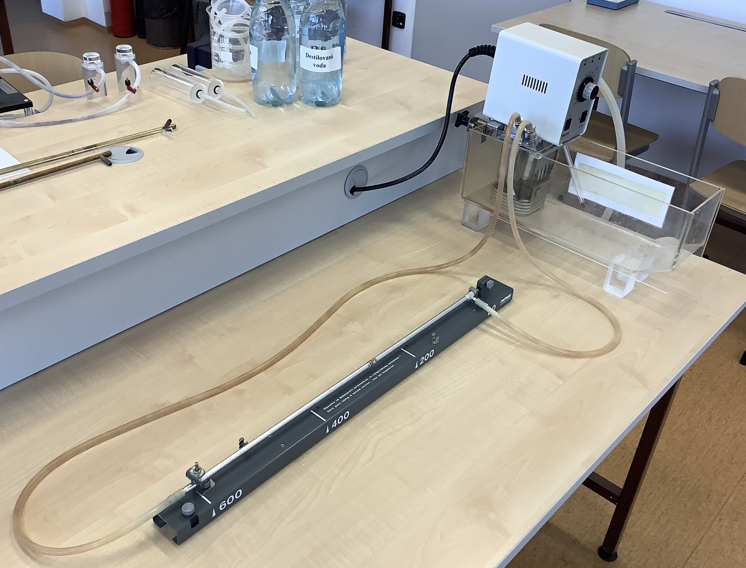
\includegraphics[width=.4\textwidth]{schema.png}
  \caption{Skutečná soustava pro měření}
  \label{fig:aparatura}
\end{figure}
\begin{figure}[htbp]
  \centering
  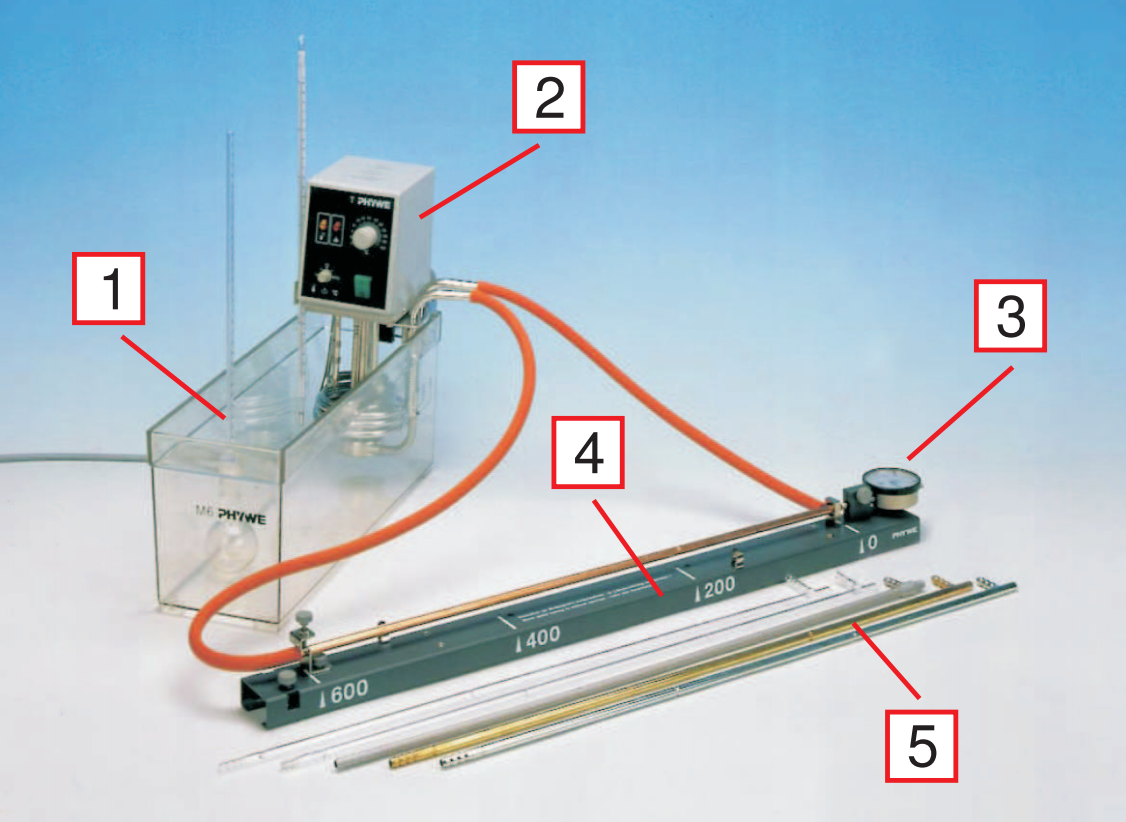
\includegraphics[width=.4\textwidth]{schema-cisla.png}
  \caption{Model aparatury}
  \label{obr:soustava}
\end{figure}

\subsection{Postup experimentu}
Stejný postup je aplikovatelný na všechny vzorky. Použitá aparatura je vidět na obrázcích \ref{obr:soustava} a \ref{fig:aparatura}.
Do nádržky s vodou (1) je umístěno topné těleso (2) s termostatem. Do lavice (4) se upevňují měřené vzorky (5) a z indikátorových hodinek (3) je odečítána měnící se délka měřeného vzorku. Předpokládáme, že teplota v celém vodním systému je stejná a že stejnou teplotu má i měřený vzorek. Zanedbáváme tak konečné tepelné vodivosti materiálů použitých v experimentu. 

\begin{enumerate}
  \item Vodní systém naplňte chladnou vodou z vodovodu až do úrovně 2 cm pod okraj nádoby s topným tělesem a termostatem. Měřený vzorek upevněte do upínací lavice, na jeho konce nasaďte přívodní hadičky pro vodu. Na konec vzorku umístěte indikátorové hodinky tak, aby se měřicí hrot dotýkal měřeného vzorku.
  \item Nastavte termostat na nejnižší teplotu, vyčkejte ustálení teplot v systému. Poznamenejte referenční teplotu $t_0$ a počáteční délku vzorku $l_0$, vůči kterým později vztáhneme absolutní proudloužení a změnu teploty. Dále se nesmí manipulovat se soustavou, aby nedošlo k posunutí indikátorových hodinek.
  \item Opakovaně navyšte teplotu na termostatu o pevný krok (pro nás 5~\degree C) a vyčkejte opětovného ustálení soustavy. Následně odečtěte novou dvojici ($t_i$, $l_i$) z teploměru a indikátorových hodinek. Opakujte až do dosažení cílové teploty (pro nás 60~\degree C).
  \item Vypněte topné těleso i čerpadlo, vodu z nádržky vypusťte. Indikátorové hodinky sundejte z upínací lavice a umístěte je do obalu. Ze systému hadiček a vnitřku vzorku nechte odtéci vodu, odpojte přívodní hadičky. Vzorek demontujte z upínací hadice. V případě potřeby měřit další vzorek opakujte postup od kroku 1.
\end{enumerate}

\subsection{Naměřené hodnoty}
Všechny naměřené hodnoty jsou v~tabulkách \ref{tab:mosaz} a \ref{tab:sklo} a grafech \ref{graph:mosaz} a \ref{graph:sklo}. Pro oba vzorky bylo provedeno deset měření, žádné měření nebylo opakováno za stejných podmínek dvakrát (nebude tudíž mít smysl uvažovat nejistoty typu A). Naměřenými dvojicemi ($t_i$, $l_i$) byla proložena lineární funkce se směrnicí $A$. Protože úpravou vztahu \eqref{eq:defalpha} získáme
\begin{equation}
  \underbrace{\frac{\Delta l}{\Delta t}}_{A} = \alpha L\text{,}
\end{equation}
je potřeba vypočtenou směrnici $A$ ještě podělit délkou vzorku $L$ určenou v zadání úkolu \ref{ch:ukoly}.

\begin{table}[htbp]
  \centering
    \centering
    \begin{tabular}[t]{|c|l|l|}
      \hline
      t [\degree C] & $\Delta l$ [$0.01~$mm] & $A_i$ [$0.01~\text{mm}\cdot\text{K}^{-1}$]\\\hline\hline
      25,7	&	0	&	---		\\\hline
      31,7	&	7	&	1,167		\\\hline
      36,8	&	12,5	&	1,126		\\\hline
      42,2	&	18,5	&	1,121		\\\hline
      46,3	&	23	&	1,117		\\\hline
      50,9	&	27,5	&	1,091		\\\hline
      56	&	33	&	1,089		\\\hline
      61,2	&	38,5	&	1,085		\\\hline
      65,7	&	44	&	1,100		\\\hline
      70,4	&	48,5	&	1,085		\\\hline
      
      \hline
      \multicolumn{3}{|c|}{$\overline{\Delta l}= 5,3\bar{8} \cdot 10^{-5}~\text{m}$}\\\hline
      \multicolumn{3}{|c|}{$\overline{\Delta t}= 4,9\bar{6}~\text{K}$}\\\hline
      \multicolumn{3}{|c|}{$A=1,081 \cdot 10^{-5}~\text{m}\cdot\text{K}^{-1}$}\\\hline
      \multicolumn{3}{|c|}{$\alpha = A/L = 1.801\bar{6} \cdot 10^{-5}~\text{K}^{-1}$}\\\hline
    \end{tabular}
    \caption{Prodloužení mosazné tyčky}
    \label{tab:mosaz}
\end{table}


\begin{graph}[htbp]
  \centering
  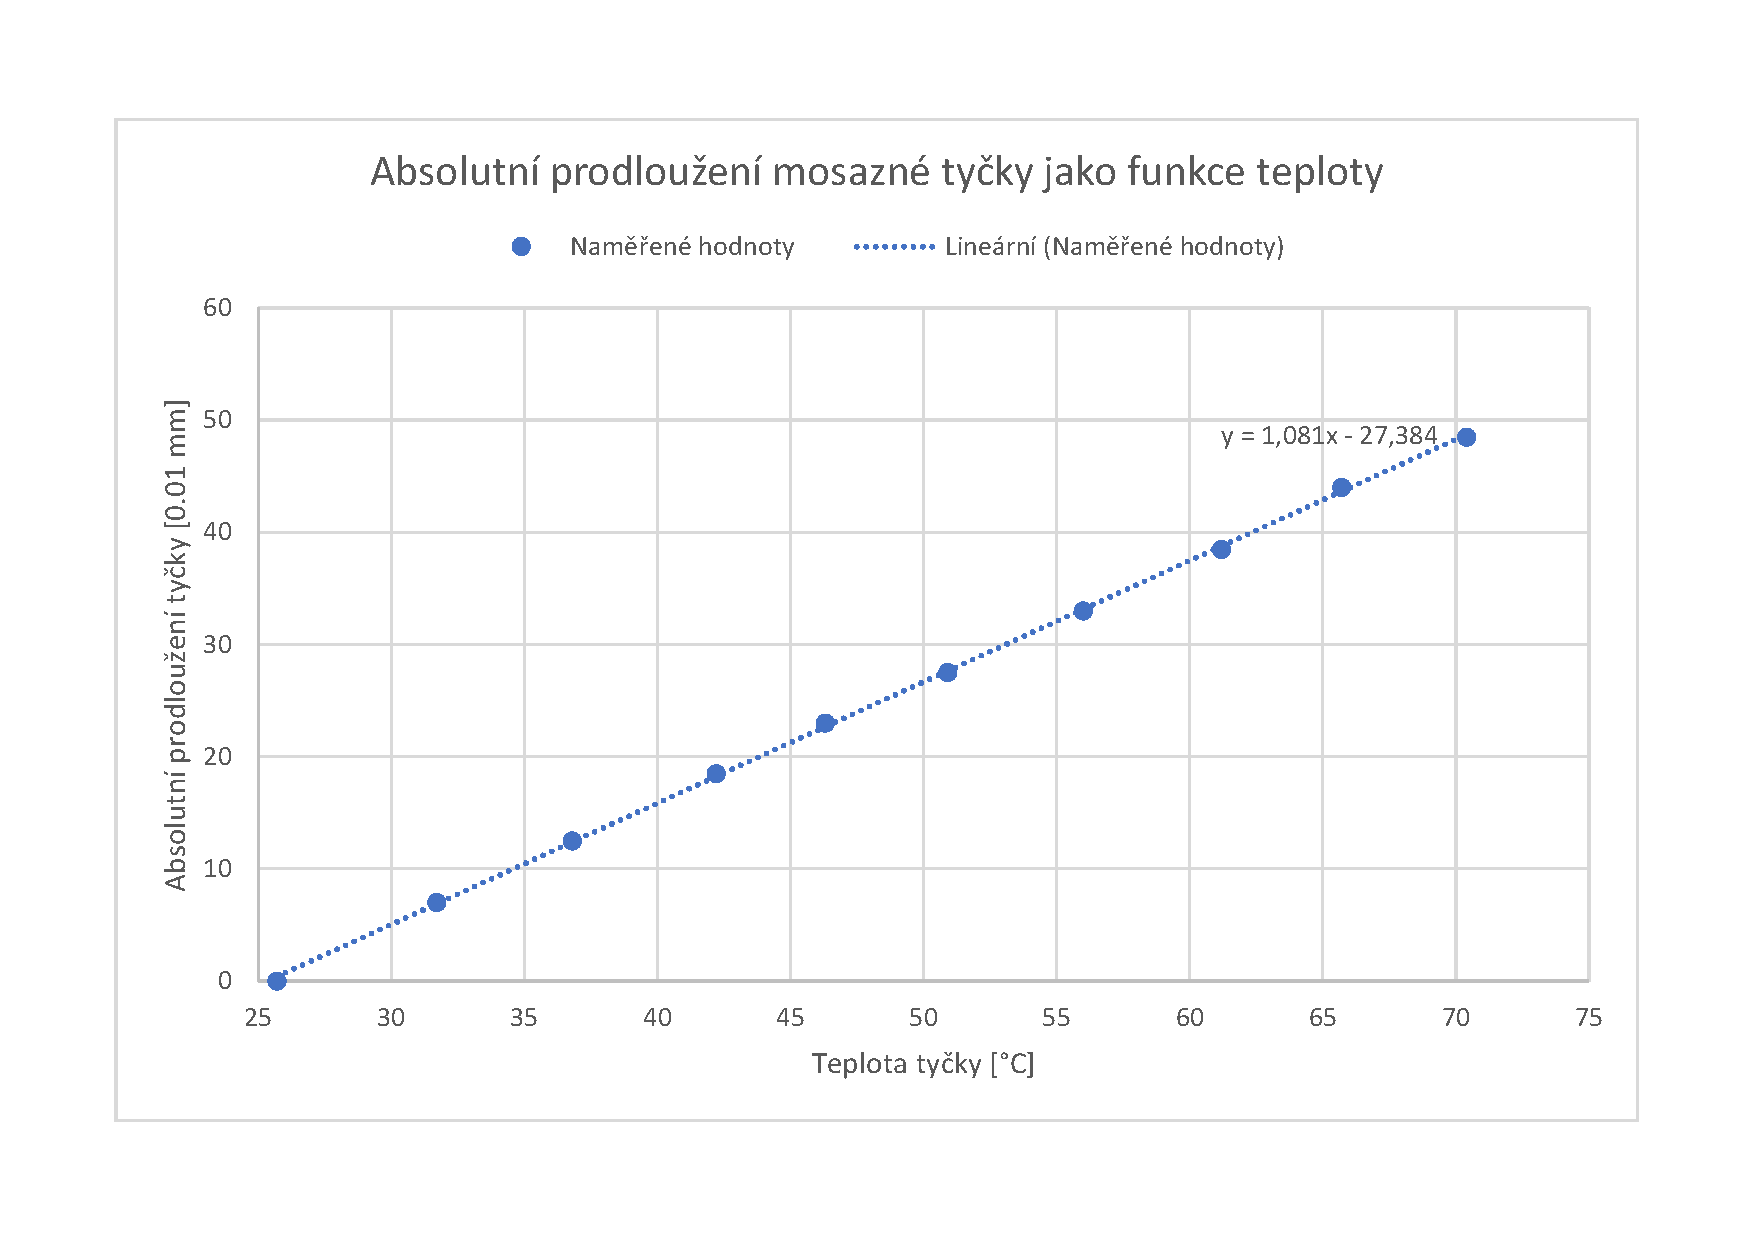
\includegraphics[width=\textwidth]{graph-brass.pdf}
  \caption{Závislost prodloužení mosazné tyčky na její teplotě}
  \label{graph:mosaz}  
\end{graph}
\begin{table}[t]
  \centering
    \centering
    \begin{tabular}[t]{|c|l|l|}
      \hline
      t [\degree C] & $\Delta l$ [$0.01~$mm] & $A_i$ [$0.01~\text{mm}\cdot\text{K}^{-1}$]\\\hline\hline
      25,3	&	0	&	---		\\\hline
      31,5	&	1,5	&	0,242		\\\hline
      36,9	&	2,3	&	0,198		\\\hline
      42,3	&	3,5	&	0,206		\\\hline
      46,8	&	4,3	&	0,200		\\\hline
      51,8	&	5	&	0,189		\\\hline
      56,5	&	6	&	0,192		\\\hline
      61,1	&	6,7	&	0,187		\\\hline
      66,1	&	7,4	&	0,181		\\\hline
      70	&	8	&	0,179		\\\hline
      
      \hline
      \multicolumn{3}{|c|}{$\overline{{\Delta l}}= 0,\bar{8} \cdot 10^{-5}~\text{m}$}\\\hline
      \multicolumn{3}{|c|}{$\overline{\Delta t}= 4,9\bar{6}~\text{K}$}\\\hline
      \multicolumn{3}{|c|}{$A=0.1769 \cdot 10^{-5}~\text{m}\cdot\text{K}^{-1}$}\\\hline
      \multicolumn{3}{|c|}{$\alpha = A/L = 0.2948\bar{3} \cdot 10^{-5}~\text{K}^{-1}$}\\\hline
    \end{tabular}
    \caption{Prodloužení skleněné tyčky}
    \label{tab:sklo}
  \end{table}
  
  \begin{graph}[htbp]
    \centering
    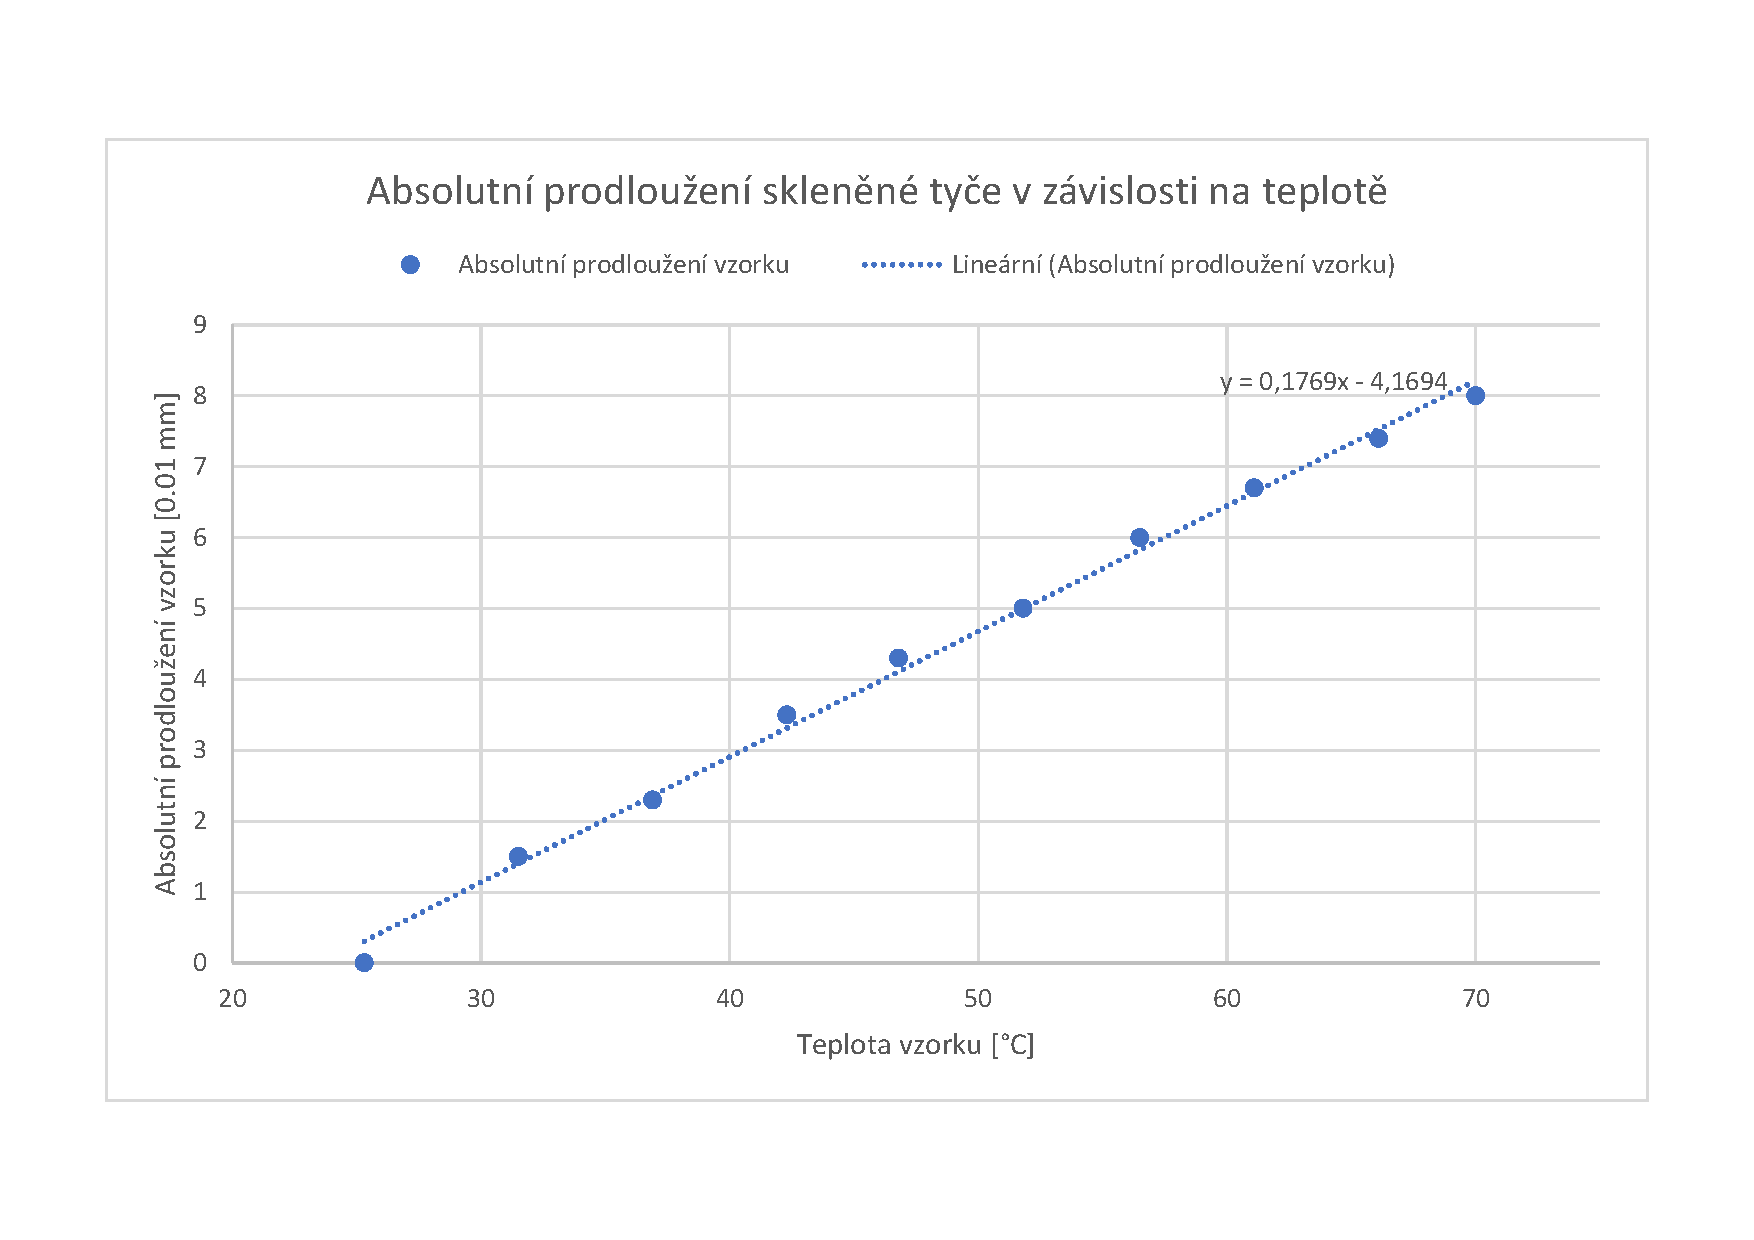
\includegraphics[width=\textwidth]{graph-glass.pdf}
    \caption{Závislost prodloužení skleněné tyčky na její teplotě}
    \label{graph:sklo}
\end{graph}
\subsection{Použité přístroje a nejistoty}
\begin{enumerate}
  \label{pristroje}
  \item Teploměr Greisinger GTH 175, nejistota měření je $\pm 0.1\%$ naměřené hodnoty $\pm 2$ digity. Protože teploměr měří na tři místa a jedno desetinné, má digit velikost $10^{-1}$. \cite{url:thermometer}
  \item Ručkový úchylkoměr Köfer M2 TOP, rozlišení 10 \textmu m \cite{url:prezentace}
\end{enumerate}

\subsection{Nejistota měření}
Každé měření bylo zatíženo chybou. Pomocí údajů ze seznamu \ref{pristroje} určíme standardní nejistoty typu C jako
\begin{equation}
  \begin{split}
    u_{\text{Cl}} &= \sqrt{0 + u^2_{\text{Bl}}} = \frac{\Delta}{\sqrt{12}} = \frac{10 \mu m}{\sqrt{12}} \approx 2.9~\text{\textmu m},\\
    u_{\text{Ct}} &= \sqrt{0 + u^2_{\text{Bt}}} =\frac{hodnota \cdot \frac{0.1}{100}+0.2}{\sqrt{3}} \le \frac{70 \cdot \frac{0.1}{100}}{\sqrt{3}} \approx 0.12 ~\degree \text{C},\\
    u_{\text{CL}} &= 1~\text{mm (podle zadání)},\\
    \label{eq:nejistoty}
  \end{split}
\end{equation}
s přihlédnutím k faktu, že měření teploty $t$ proběhlo digitálním teploměrem, zatímco indikátorové hodinky měřící délku $\Delta l$ byly ručkový měřicí přístroj. Nejvyšší dosažená teplota byla 70~\degree C, odtud plyne horní odhad pro nejistotu $u_\text{Bt}$. Kvůli absenci vícenásobných měření za týchž podmínek nemá cenu hovořit o standardní nejistotě typu A $u_\text{A}$ a kombinovaná nejistota se rovná nejistotě vypočtené metodou B.

Pomocí zákona šíření nejistot podle \cite{url:konicek} hledáme kombinovanou standardní nejistotu $u_\text{C}(\alpha)$ jako
\begin{equation}
    u_\text{C}(\alpha) = \sqrt{\left(\frac{\partial \alpha}{\partial \Delta t}\right)_{L, \overline{\Delta t}, \overline{\Delta l}}^2u^2_{\text{Ct}}+\left(\frac{\partial \alpha}{\partial \Delta l}\right)_{L, \overline{\Delta t}, \overline{\Delta l}}^2u^2_{\text{Cl}}+\left(\frac{\partial \alpha}{\partial L}\right)_{L, \overline{\Delta t}, \overline{\Delta l}}^2u^2_{\text{CL}}},\\
    \label{eq:nejistotamain}
  \end{equation}
  kam do \textit{koeficientů citlivosti} dosadíme střední hodnoty veličin $L$, $\Delta t$, $\Delta l$ vypočtené v tabulkách \ref{tab:mosaz} a \ref{tab:sklo}.


  \begin{equation}
    u_\text{C}(\alpha) = \sqrt{\left(\frac{- \overline{\Delta l}}{L (\overline{\Delta t})^2}\right)^2u^2_{\text{Ct}}
    +\left(\frac{1}{L\overline{\Delta t}}\right)^2u^2_{\text{Cl}}
    +\left(\frac{- \overline{\Delta l}}{L^2 \overline{\Delta t}}\right)^2u^2_{\text{CL}}},\\
  \end{equation}
  po dosazení vyjde 
  \begin{equation}
    \begin{split}
      u_\text{C}(\alpha_{mosaz}) = 1,0681 \cdot 10^{-6}\text{K}^{-1}\text{,} \\
      u_\text{C}(\alpha_{sklo}) = 0,121198 \cdot 10^{-6}\text{K}^{-1}\text{.}
    \end{split}
  \end{equation}

\begin{table}[htbp]
  \centering
  \begin{tabular}{|l|l|}
    \hline
    Mosazná tyč & $\alpha_{mosaz} = (18,01 \pm 1,06) \cdot 10^{-6} \text{K}^{-1}$\\\hline
    Skleněná tyč & $\alpha_{sklo} = (2,948 \pm 0,121) \cdot 10^{-6} \text{K}^{-1}$\\\hline
  \end{tabular}
  \caption{Výsledné hodnoty s chybami na tři platná místa}
  \label{tab:final}
\end{table}

\subsection{Diskuse}
\label{ch:diskuze}
Naměřená hodnota součinitele teplotní roztažnosti mosazi odpovídá tabulkové hodnotě v řádu $10^{-5}$ i $10^{-6}$, v žádných tabulkách se mi nepodařilo nalézt $\alpha_{mosaz}$ s přesností vyšší než na dvě platná místa, nemohu tedy příliš soudit o přesnosti měření porovnáním s tabulkovou hodnotou. Ani u skla nelze snadno srovnávat, neboť neznáme jeho přesný typ. Podle \cite{url:sklo} se typické koeficienty $\alpha$ pro sklo pohybují v řádu $3\cdot 10^{-6} \text{K}^{-1}$ až $10 \cdot 10^{-6}\text{K}^{-1}$, kam náš výsledek řádově spadá. Mohlo by se jednat o sklo laboratorní, u nějž očekávám co největší odolnost proti změnám teploty a tudíž i nízkou teplotní roztažnost.

Znepokojivá je vysoká chyba měření, která má potenciál zneplatnit poslední platnou číslici. Je způsobena zejména faktickými problémy našeho modelu - tyč se neprohřívá ve skutečnosti všude stejně a ideálně rychle, navíc je vodou protékána jen na své vnitřní straně, vliv tak může mít i nenulový rozdíl teplot mezi vnějším a vnitřním povrchem materiálu. Pro vyšší přesnost měření by bylo vhodné měřený vzorek celý do lázně ponořit a dát mu více času na srovnání teplot s lázní. V neposlední řadě by chybě pomohlo použití teploměru s vyšší přesností, protože podle rovnic \eqref{eq:nejistoty} je to z celého experimentu nejméně přesné měření.

\section{Závěr}
\label{ch:zaver}
Zpracovali jsme naměřená data, vypočetli koeficient tepelné roztažnosti a~určili nejistoty pro mosaznou a skleněnou tyč. Pro mosaz vyšla velice přesně tabulková hodnota, ovšem s vysokou relativní chybou 5,5~\%. Pro sklo vyšla hodnota v rozsahu typických hodnot pro sklo, relativní chyba jsou 4~\%.

Z dílčích nejistot ze vzorce \ref{eq:nejistotamain} se jako zdroj největší chyby ukazuje digitální teploměr, další chyba je způsobena chybami v modelu fyzikálního experimentu.

%--- LITERATURA a~ZDROJE (povinne) ---
\clearpage
\renewcommand{\refname}{Seznam použité literatury a~zdrojů informací} 
%\section*{Seznam použité literatury a~zdrojů informací}
\phantomsection %pridej odkaz do PDF zalozek
\addcontentsline{toc}{section}{Seznam použité literatury a~zdrojů informací}

\begin{thebibliography}{99}

%----------------------------------------------------
\subsection*{Seznam použitých internetových zdrojů}
    \bibitem{url:navod} \url{http://herodes.feld.cvut.cz/mereni/downloads/navody/roztaznost.pdf} [cit.~25.~listopadu~2020]
    \bibitem{url:thermometer} \url{http://herodes.feld.cvut.cz/mereni/downloads/manualy/GTH175Pt.pdf} [cit.~18.~listopadu~2020]
    \bibitem{url:prezentace} \url{http://aldebaran.feld.cvut.cz/vyuka/konicek/F2-B1B02FY2/laborky/07.%20Mereni%20teplotniho%20soucinitele%20delkove%20roztaznosti/tepl_roztaznost%20-%20Prezentace.odp} [cit.~3.~listopadu~2020]
    \bibitem{url:konicek} \url{http://aldebaran.feld.cvut.cz/vyuka/konicek/nejistoty/slajdy-nejistoty.html} [cit.~3.~listopadu~2020]
    \bibitem{url:sklo} \url{http://www.glassrevue.com/news.asp@nid=1174&cid=6.html} [cit.~27.~listopadu~2020]
\end{thebibliography}

\end{document}